\documentclass[9pt]{beamer}
\usepackage{styles/mypreamble}
%~~~~~~~~~~~~~~~~~~~~~~~~~~~~~~~~~~~~~~~~~~~~~~~~~~~~~~~~~~~~~~~~~~~~~~~~~~~~~~
\title{Алгоритмы машинного обучения}
\subtitle{Лекция 2. Методы оптимизации}
\author{Владимир Кукушкин}
\institute{СПбГЭУ - 18.11.2020}
%~~~~~~~~~~~~~~~~~~~~~~~~~~~~~~~~~~~~~~~~~~~~~~~~~~~~~~~~~~~~~~~~~~~~~~~~~~~~~~

\begin{document}

\titlepage

\section{Градиентный спуск}
\begin{frame}{Постановка задачи}
\begin{itemize}
    \item Пусть есть дифференцируемая функция $f(x): \mathbb{R}^n \rightarrow \mathbb{R}$.
    \item Хотим найти её минимум.
\end{itemize}
\end{frame}

\begin{frame}{Идея алгоритма}
    \begin{itemize}
        \item Знаем, что вектор-градиент функции в точке указывает в направлении наибольшего роста функции.
        $$\mathop{\nabla} f(x)\big|_{x=a} = \left(\frac{\partial f}{\partial x_1}, \ldots, \frac{\partial f}{\partial x_n}\right)\Big|_{x_1=a_1, \ldots x_n=a_n}.$$
        \item Значит, если сдвинуть точку $a$ в направлении антиградиента (со знаком минус), то значение функции в новой точке скорее всего уменьшится:
        \item Но это не точно. Всё зависит от шага и от характера самой функции в окрестности точки. Однако, если правильно выбирать сдвиг (например, делать его достаточно маленьким), то можно постепенно сходиться к минимуму.
    \end{itemize}
\end{frame}

\begin{frame}{Градиентный спуск. Постоянный шаг.}
\begin{enumerate}
    \item Выбираем $\alpha$ (a.k.a. learning rate). Встаём в произвольную точку $x^{(0)}$.
    \item Вычисляем градиент функции в этой точке $\mathop{\nabla}^{(k)} = \mathop{\nabla} f(x)\big|_{x=x^{(k)}}$.
    \item Сдвигаем точку $x^{(k+1)} = x^{(k)} - \alpha \mathop{\nabla}^{(k)}$:
    \begin{center}
        \begin{tabular}{c}
             $x^{(k+1)}_1 = x^{(k)}_1 - \alpha \frac{\partial f}{\partial x_1}\big|_{x_1 = x^{(k)}_1}$\\
             $\cdots$\\
             $x^{(k+1)}_n = x^{(k)}_n - \alpha \frac{\partial f}{\partial x_n}\big|_{x_n = x^{(k)}_n}$\\
        \end{tabular}
    \end{center}
    \item Повторять пп. 2, 3 до сходимости. 
\end{enumerate}

Признаки сходимости (критерии останова):
\begin{itemize}
    \item $\|x^{(k+1)} - x^{(k)}\| < \varepsilon$,
    \item $\|f(x^{(k+1)}) - f(x^{(k)})\| < \varepsilon$.
\end{itemize}
\end{frame}

\framedgraphic{Иллюстрация}{img/gradient_descent.png}

% \framedgraphic{Выбор шага}{img/gradient_descent_learning_rate.png}


\begin{frame}{Выбор шага}
\begin{center}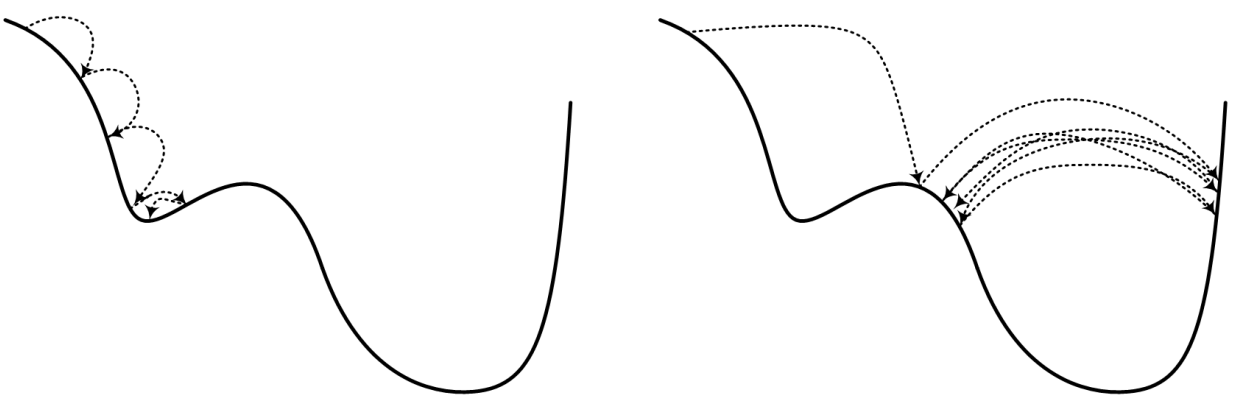
\includegraphics[height=120px, width=\textwidth]{img/gradient_descent_learning_rate.png}\end{center}
\begin{itemize}
    \item Уже говорилось, что $\alpha$ надо подбирать разумно.
    \item При слишком маленьких $\alpha$ можно очень долго сходиться к экстремуму.
    \item При слишком больших $\alpha$ можно не попасть в экстремум.
\end{itemize}
\end{frame}

\begin{frame}{Выбор шага. Наивный подход.}
    \begin{itemize}
        \item Скорее всего, на первый итерациях мы будем достаточно далего от экстремума. Поэтому разумно вначале идти с более крупным шагом и уменьшать его по мере приближения к экстремуму.
        \item Обратно пропорционально номеру итерации: $\alpha^{(k)} = \gamma\frac{\alpha^{(0)}}{k}$.
        \item Экспонентно-затухающий шаг: $\alpha^{(k)} = \alpha^{(0)}e^{-\gamma k}$.
        \item Наивность подхода в том, что он совсем не учитывает характер оптимизируемой функции. Легко может оказаться, что мы слишком рано сделаем шаг слишком маленьким, и перестанем приближаться к экстремуму.
    \end{itemize}
\end{frame}

\begin{frame}{Метод импульсов}
\begin{itemize}
    \item Идея в том, что на каждой итерации будем менять направление не целиком на то, которое предлагает новый градиент, а будем частично сохранять движение вдоль предыдущего градиента тоже. Аналогия с изменением движения точки, имеющей массу: благодаря инерции она будет сохранять предыдущее направление движения.
    \item Пусть $v^{(k-1)}$ -- вектор сдвига точки на предыдущем $(k-1)$-м шаге. Тогда 
    $$v^{(k)} = \gamma v^{(k-1)} - \alpha \mathop{\nabla^{(k)}},$$
    где параметр $\gamma \in [0, 1]$ регулирует сохранение предыдущего направления движения.
    $$x^{(k)} = x^{(k-1)} + v^{(k)}.$$
\end{itemize}
\end{frame}

\begin{frame}{Метод Нестерова}
\begin{itemize}
    \item Модификация метода импульсов: считаем градиент не в точке $x^{(k)}$, а в точке $x^{(k)} + \gamma v^{(k-1)}$, в которую мы бы сместились по инерции:
    $$v^{(k)} = \gamma v^{(k-1)} - \alpha \mathop{\nabla f(x)} \Big|_{x=x^{(k)} + \gamma v^{(k-1)}},$$
    $$x^{(k)} = x^{(k-1)} + v^{(k)}.$$
\end{itemize}
\end{frame}

\begin{frame}{Плюсы, минусы, подводные камни}
\begin{itemize}
    \item Универсальный алгоритм. Применяется повсеместно в ML (особенно в нейронных сетях).
    \item Сходится лишь к локальному экстремуму.
    \item Требует знания производной минимизируемой функции (не обязательно: достаточно уметь считать её численно).
\end{itemize}
    
\end{frame}
\section{EM-алгоритм}
\begin{frame}{Задача о разделении гауссовской смеси}
\begin{itemize}
    \item EM-алгоритм проще объяснить на примере конкретной задачи.
    \item Пусть $Y_1 \sim \mathcal{N}(\underbrace{\mu_1, \sigma_1^2}_{\theta_1}) = \phi(\theta_1)$ и $Y_2 \sim \mathcal{N}(\underbrace{\mu_2, \sigma_2^2}_{\theta_2}) = \phi(\theta_2)$.\newline
    $\mu_1, \mu_2, \sigma_1^2, \sigma_2^2$ -- неизвестные параметры.
    \item Пусть у нас есть выборка из смеси этих распределений $$Y = (1-\Delta)\cdot Y_1 + \Delta\cdot Y_2,$$ где $\Delta \in \{0, 1\}$ и $\text{Pr}(\Delta = 1) = \pi$ -- также неизвестный параметр.  
    \item Задача: по выборке из $Y$ оценить параметры $\theta=(\pi, \mu_1, \sigma_1^2, \mu_2, \sigma_2^2)$.
    \item Картинка для трёх смесей (у нас только две), но больно  хороша.
\end{itemize}
\begin{center}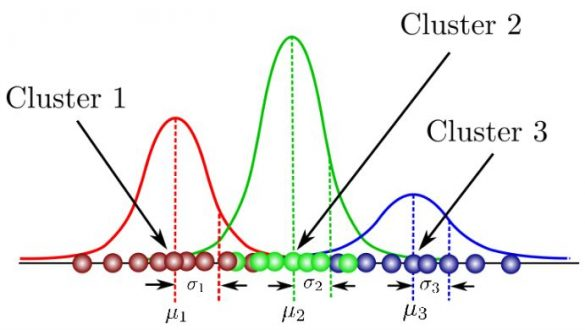
\includegraphics[height=100px]{img/gaussian_mixture_em.jpg}\end{center}
\end{frame}

\begin{frame}{Идея. Часть 1. Метод максимального правдоподобия.}
\begin{itemize}
    \item Плотность $Y$ имеет вид:
    $$g_Y(y) = (1-\pi)\phi_{\theta_1} + \pi\phi_{\theta_2}$$
    \item Тогда правдоподобие наблюдать данные из выборки записывается как
    $$L(\theta) = \prod_{i=1}^N [(1-\pi)\phi_{\theta_1} + \pi\phi_{\theta_2}],$$
    а его логарифм как
    $$l(\theta) = \sum_{i=1}^N \log[(1-\pi)\phi_{\theta_1} + \pi\phi_{\theta_2}].$$
    \item Теперь надо как-то максимизировать правдоподобие $l(\theta)$, но это сложно сделать в лоб из-за сложных логарифмов сумм.
\end{itemize}
\end{frame}

\begin{frame}{Идея. Часть 2. EM-алгоритм.}
    \begin{itemize}
        \item Что если мы знали бы \textit{точно} все реализации $\Delta_i$ (то есть для каждого $i$ знали бы значение $\Delta_i$ = 1 или $\Delta_i$ = 0)?
        \item Тогда мы бы разбили всю выборку всю выборку $y_i$ (множество её индексов) на две:
        $$I_1 = \{i \;|\; i: \Delta_i=0\} \text{ и } I_2 = \{i \;|\; i: \Delta_i=1\},$$
        и тогда оценивали $(\mu_1, \sigma_1^2)$ и $(\mu_2, \sigma_2^2)$ по этим выборкам по-отдельности (как среднее и выборочнкую дисперсию):
        \begin{equation}\label{em_mu_sigma}
            \begin{split}
            \hat\theta_1: \;\;\;\;\;\; \hat\mu_1 = \frac{\sum\limits_{i\in I_1} y_i}{|I_1|}  \text{  ,  } \hat\sigma_1^2 = \frac{\sum\limits_{i\in I_1} (y_i - \hat\mu_1)^2}{|I_1|},\\
            \hat\theta_2: \;\;\;\;\;\; \hat\mu_2 = \frac{\sum\limits_{i\in I_2} y_i}{|I_2|}  \text{  ,  } \hat\sigma_2^2 = \frac{\sum\limits_{i\in I_2} (y_i - \hat\mu_1)^2}{|I_2|}.
            \end{split}
        \end{equation}
        \item Но как понять где $\Delta_i=0$, а где $\Delta_i = 1$?
    \end{itemize}
\end{frame}

\begin{frame}{Идея. Часть 3. Как определять $\Delta_i$.}
    \begin{itemize}
        \item Пусть у нас есть какие-то оценки $\hat\pi, \hat\theta_1, \hat\theta_2$. Точность оценок пока не волнует. Начать можно с $\hat\pi = 0.5$, $\hat\mu_1 = \hat\mu_2 = \sum_{i=1}^N y_i/N$, $ \hat\sigma_1^2=\hat\sigma_2^2=\sum_{i=1}^N (y_i - \bar y)^2/N$.
        \item Тогда можно посчитать в каждой точке $i$, что более правдоподобнее: что точка из $Y_1$ или из $Y_2$. А именно, посчитать отношение плотностей:
        $$\text{Pr}(\Delta_i=1|\theta) = \hat\gamma_i = \frac{\hat\pi \phi_{\hat\theta_2}(y_i)}{(1-\hat\pi) \phi_{\hat\theta_1}(y_i) + \hat\pi \phi_{\hat\theta_2}(y_i)}.$$
        В числителе значение плотности второй компоненты смеси, в знаменателе -- всей смеси. Чем ближе $\hat\gamma_i$ к 1, тем вероятнее, что $y_i$ выбран из второй компоненты смеси.
        \item Теперь, зная $\hat\gamma_i$ можно уточнить $\hat\theta_1$, $\hat\theta_2$ по аналогии с формулами \eqref{em_mu_sigma}, только беря взвешенные средние с весами $(1-\hat\gamma_i)$ для $\theta_1$ и $\hat\gamma_i$ для $\theta_2$.
        \item И наконец, уточнить $\hat\pi = \sum_{i=1}^N\hat\gamma_i/N$.
    \end{itemize}
\end{frame}

\begin{frame}{Итоговый алгоритм}
    \begin{enumerate}
        \item Берём начальные приближения для $\hat\pi, \hat\mu_1, \hat\mu_2, \sigma_1^2, \sigma_2^2$.
        \item Expectation шаг (E-step): считаем вероятности $\text{Pr}(\Delta_i=1|\theta)$:
        $$\hat\gamma_i = \frac{\hat\pi \phi_{\hat\theta_2}(y_i)}{(1-\hat\pi) \phi_{\hat\theta_1}(y_i) + \hat\pi \phi_{\hat\theta_2}(y_i)}.$$
        \item Maximization-шаг (M-step): Уточняем $\hat\pi, \hat\mu_1, \hat\mu_2, \sigma_1^2, \sigma_2^2$:
        \begin{gather*}
        \hat\mu_1 = \frac{\sum\limits_{i=1}^N (1-\hat\gamma_i)y_i}{\sum\limits_{i=1}^N (1-\hat\gamma_i)}  \text{  ,  } \hat\sigma_1^2 = \frac{\sum\limits_{i=1}^N (1-\hat\gamma_i)(y_i - \hat\mu_1)^2}{\sum\limits_{i=1}^N (1-\hat\gamma_i)},\\
        \hat\mu_2 = \frac{\sum\limits_{i=1}^N \hat\gamma_i y_i}{\sum\limits_{i=1}^N \hat\gamma_i}  \text{  ,  } \hat\sigma_2^2 = \frac{\sum\limits_{i=1}^N \hat\gamma_i(y_i - \hat\mu_2)^2}{\sum\limits_{i=1}^N \hat\gamma_i},\\
        \hat\pi = \frac{\sum\limits_{i=1}^N \hat\gamma_i}{N}.
        \end{gather*}
        \item Повторить шаги 2,3 до сходимости.
    \end{enumerate}
\end{frame}

\begin{frame}{EM-алгоритм. Обобщение.}
    \begin{itemize}
        \item Если нужно оптимизировать сложную функцию, то можно "съесть слона по кусочкам".
        \item Задаём начальное приближение параметров (хоть случайно).
        \item Expectation-шаг (E-step). Фиксируем часть параметров из общих соображений.
        \item Maximization-шаг (M-step). Оптимизируем оставшиеся параметры. 
        \item Повторяем E, M шаги до сходимости.
    \end{itemize}
\end{frame}

\end{document}